\documentclass{article} % For LaTeX2e
\usepackage{nips14submit_e,times}
\usepackage{hyperref}
\usepackage{url}
\usepackage{amsmath}
\usepackage{graphicx,float,wrapfig}
\usepackage{caption}
\usepackage{subcaption}
\usepackage{natbib}
	\usepackage{bibhacks}
\usepackage[nowarn]{glossaries}
%\documentstyle[nips13submit_09,times,art10]{article} % For LaTeX 2.09

% Use these acronyms instead of writing PMF or Probabilistic Matrix Factorization
% They take care of doing Probabilistic Matrix Factorization (PMF) the first
% time it is mentioned, etc...
\glsdisablehyper
\newacronym{pmf}{PMF}{Probabilistic Matrix Factorization}
\newacronym{lda}{LDA}{Latent Dirichlet Allocation}
\newacronym{bpf}{BPF}{Bayesian Poisson Factorization}
\newacronym{hpf}{HPF}{Hierarchical Poisson Factorization}
\newacronym{cf}{CF}{Collaborative Filtering}
\newacronym{svd}{SVD}{Singular Value Decomposition}
\newacronym{mcmc}{MCMC}{Markov Chain Monte Carlo}
\newacronym{pf}{PF}{Poisson Factorization}

\title{Probabilistic Matrix Factorization}


\author{ 
  Mert Terzihan \\
  Department of Computer Science\\
  Brown University\\
  Providence, RI 02912 \\
  \texttt{mert\_terzihan@brown.edu}
  \And
  Gabriel Barth-Maron \\
  Department of Computer Science \\
  Brown University \\
  Providence, RI 02912 \\
  \texttt{gabriel\_barth-maron@brown.edu}\\
}

% The \author macro works with any number of authors. There are two commands
% used to separate the names and addresses of multiple authors: \And and \AND.
%
% Using \And between authors leaves it to \LaTeX{} to determine where to break
% the lines. Using \AND forces a linebreak at that point. So, if \LaTeX{}
% puts 3 of 4 authors names on the first line, and the last on the second
% line, try using \AND instead of \And before the third author name.

\newcommand{\fix}{\marginpar{FIX}}
\newcommand{\new}{\marginpar{NEW}}

\nipsfinalcopy % Uncomment for camera-ready version

\begin{document}


\maketitle
\begin{abstract}
This is an abstract.
\end{abstract}

\section{Introduction}
\Gls{pmf} is an approximate way to factorize a matrix. In another way, product 
of the matrices that were produced by factorization is an approximation of the 
original matrix. This set of algorithms utilize probabilistic modeling to tackle 
the problem of decomposing matrices. For datasets that are big enough, the 
deterministic methods (i.e \Gls{svd}) could be infeasible to apply. \Gls{pmf} 
models can be learned by EM, \Gls{mcmc}, or as it has been proposed with recent 
research, Variational methods. 

One application of \Gls{pmf} is recommendation systems. Recommendation systems 
aim to produce recommendations to users based on their previous choices and/or 
their demographic information. The interactions between users and items can be 
represented in matrix format, where cell $u,i$ corresponds to the relationship 
between user $u$ and item $i$. The user preferences can be modeled with some 
latent factors. By decomposing the user-item matrix into a product of two 
matrices, we can learn the factors that determine the users' decisions and thus 
cluster users and movies based on these factors. Moreover, artificial 
recommendations can be easily produced with generative models. 

The goal of this paper is to investigate different methods to tackle \Gls{pmf} 
problem especially on movie recommendations, where the interactions between 
users and movies are the ratings that are assigned by users to some movies. Note 
that the corresponding matrix can be sparse, thus making deterministic methods 
inapplicable. The paper is organized as follows: in section 2, we review the 
previous methods that were presented. In section 3, we present an extended 
version of \Gls{lda} model to use ratings as observations instead of bag-of-words 
model. In section 4, we introduce a Gibbs sampler to learn a \Gls{bpf} model. 
The results that have been obtained by learning these two models on 
\textit{MovieLens} dataset, are shared in section 5.

\section{Related Work}

\Gls{pmf} has been used extensively and to success in \gls{cf} systems \cite{koren2009matrix}. Some notable techniques that have been used in this area are: Probabilistic Latent Semantic Analysis (PLSA) \cite{hofmann1999probabilistic}, Multinomial Principal Component Analysis \cite{buntine2002variational}, \acrfull{lda} \cite{lda}, and \acrfull{bpf} \cite{gopalan2013scalable}.

\Gls{lda} is one of the most widely used matrix factorization technique in
\gls{cf} systems. As studied in \cite{lda} and \cite{discrete-pca},
one can observe that LDA is equivalent to factorizing a matrix
probabilistically using a graphical model representation. Instead of dealing with a co-occurence matrix, we will try to propose a model and
a learning algorithm to factorize a matrix where each cell is a rating of an item
by a particular user. Therefore, in addition to LDA, we would also like to generate
ratings that have been assigned by users to each item. 

In \cite{Argwal-fDLA} a method based on LDA is proposed to produce personalized recommendations.
However, fLDA takes into account much more information about the user, i.e. age, 
gender, zipcode, etc. We are going to use a simpler model, which relies on
much less personal information. We will be using only the ratings 
that have been given by the users to specific items.

A LDA-based probabilistic matrix factorization models is proposed in
\cite{conf/icdm/ShanB10}, however instead of using discrete distribution
for generating ratings, it has placed a Gaussian distribution over the user's
ratings. In our investigation we hope to relax this assumption and look into
models that are not necessarily Gaussian.

\acrfull{hpf} \cite{gopalan2013scalable} is a recent \gls{pmf} technique that
extends the Gamma-Poisson (GaP) model proposed by \cite{canny2004gap}.
In addition to \gls{hpf}, the authors of \cite{gopalan2013scalable} also
proposed \gls{bpf}, which sets the rate parameter for the Gamama distributions for
all users and items. It is believed that Poisson factorization better captures
preferences in \gls{cf} tasks. This is proven empirically, as \gls{hpf} and \gls{bpf} perform better than \gls{lda} across a variety of \gls{cf} tasks, including movie recommendation \cite{gopalan2013scalable}.


\section{\acrlong{lda}}

\section{\acrlong{bpf}}
\acrlong{bpf} is a particular model belonging to the more general class of \gls{pf} models. Similar to \gls{lda}, \gls{pf} algorithms are probabilistic models where each item $i$ is represented by $K$ latent topics, and each user $u$ can also be represented by their preferences over these latent topics \citep{gopalan2013scalable}.

\begin{align*}
	\xi_u &\sim \mathrm{Gamma}\left( a', \frac{a'}{b'} \right) \\
	\theta_{uk} &\sim \mathrm{Gamma}\left( a, \xi_u \right) \\
	\eta_i &\sim \mathrm{Gamma}\left( c', \frac{c'}{d'} \right) \\
	\beta_{ik} &\sim \mathrm{Gamma}\left( c, \eta_i \right) \\
	y_{ui} &\sim \mathrm{Poisson}\left( \theta^\top_u \beta_i \right )
\end{align*}

\begin{figure}[h]
\begin{center}
	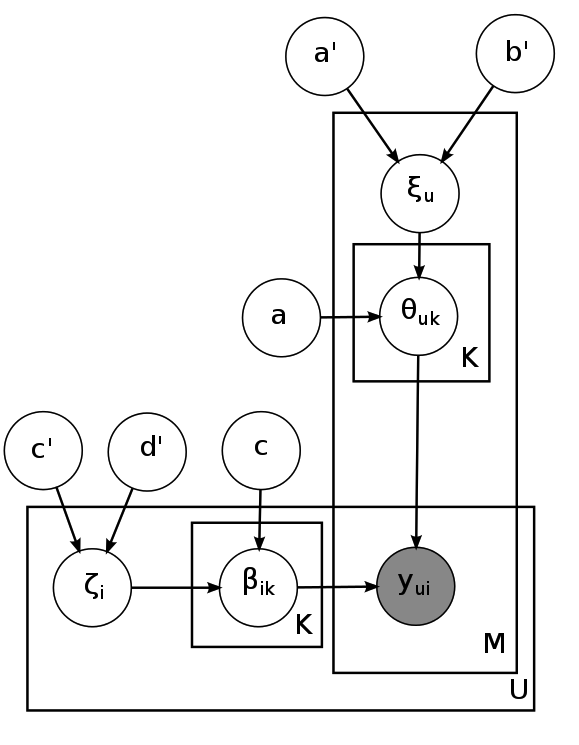
\includegraphics[scale=0.25]{bpf.png}
\end{center}
\caption{\acrlong{bpf} plate diagram}
\label{fig:bpf-model}
\end{figure}

\section{Results}

\section{Conclusions}

\section{Future Remarks}

\bibliographystyle{plain}
\bibliography{main}
\end{document}
